\documentclass{standalone}
\usepackage[dvipsnames,svgnames,x11names]{xcolor}
\usepackage{tikz}
\usepackage{pgfplots}
\pgfplotsset{compat = 1.12}
\usepackage{../thesismath}
\begin{document}
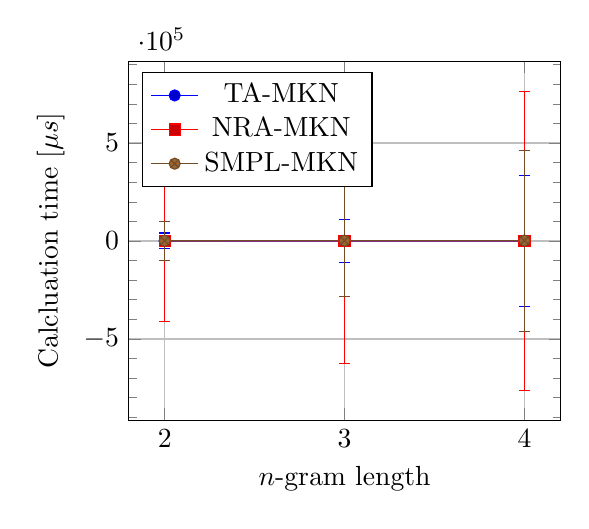
\begin{tikzpicture}[baseline]

\begin{axis}[
  xlabel = {$n$-gram length},
  xtick = {2, ..., 4},
  ylabel = {Calcluation time [${\mu}s$]},
  minor y tick num = 4,
  grid = major,
  legend entries = {{TA-MKN}, {NRA-MKN}, {SMPL-MKN}},
  legend pos = north west,
  scale = 0.8,
]

% TA-MKN
\addplot+[
  error bars/.cd,
  y dir = both,
  y explicit,
] table[y error = us_error] {
  n  us     us_error
  2    .880   40544
  3  12.596  109800
  4  76.195  332309
};

% NRA-MKN
\addplot+[
  error bars/.cd,
  y dir = both,
  y explicit,
] table[y error = us_error] {
  n  us      us_error
  2  358.575  412311
  3  669.639  626573
  4  818.547  762427
};

% NRA-MKN
\addplot+[
  error bars/.cd,
  y dir = both,
  y explicit,
] table[y error = us_error] {
  n  us      us_error
  2 1246.684  100401
  3 1749.752  285003
  4 2022.604  461763
};

\end{axis}

\end{tikzpicture}
\end{document}
